\documentclass[9pt]{article}
\usepackage[top=3cm, bottom=3cm, outer=3cm, inner=3cm]{geometry}
\usepackage{multicol}
\usepackage{graphicx}
\usepackage{url}
\usepackage{hyperref}
\usepackage{array}
\newcolumntype{x}[1]{>{\centering\arraybackslash\hspace{0pt}}p{#1}}
\usepackage{natbib}
\usepackage{multirow}
\usepackage[normalem]{ulem}
\useunder{\uline}{\ul}{}
\usepackage{listings}
\lstdefinestyle{ascii-tree}{
    literate={├}{|}1 {─}{--}1 {└}{+}1 
  }
\lstset{basicstyle=\ttfamily,
  showstringspaces=false,
  commentstyle=\color{red},
  keywordstyle=\color{blue}
}
\usepackage{caption}
\usepackage{subcaption}
\usepackage{float}
\usepackage{array}
\usepackage{longtable}
\usepackage{tabularx}
\usepackage{adjustbox}
\usepackage[table]{xcolor}% http://ctan.org/pkg/xcolor
\usepackage{blindtext}
\renewcommand{\familydefault}{\sfdefault}
\usepackage{geometry}
 \geometry{
 a4paper,
 total={190mm,257mm},
 left=10mm,
 top=20mm,
 }
\newcolumntype{M}[1]{>{\centering\arraybackslash}m{#1}}
\newcolumntype{N}{@{}m{0pt}@{}}
%%%%%%%%%%%%%%%%%%%%%%%%%%%%%%%%%%%%%%%%%%%%%%%%%%%%%%%%%%%%%%%%%%%%%%%%%%%%
%%%%%%%%%%%%%%%%%%%%%%%%%%%%%%%%%%%%%%%%%%%%%%%%%%%%%%%%%%%%%%%%%%%%%%%%%%%%
\newcommand{\itemCourse}{Estructura de Datos y Algoritmos}
\newcommand{\itemUniversity}{Universidad Nacional de San Agustín de Arequipa}
\newcommand{\itemFaculty}{Facultad de Ingeniería de Producción y Servicios}
\newcommand{\itemDepartment}{Departamento Académico de Ingeniería de Sistemas e Informática}
\newcommand{\itemSchool}{Escuela Profesional de Ingeniería de Sistemas}
\newcommand{\itemPracticeNumber}{04}
\newcommand{\itemTheme}{Sort y Listas Enlasadas}
%%%%%%%%%%%%%%%%%%%%%%%%%%%%%%%%%%%%%%%%%%%%%%%%%%%%%%%%%%%%%%%%%%%%%%%%%%%%
%%%%%%%%%%%%%%%%%%%%%%%%%%%%%%%%%%%%%%%%%%%%%%%%%%%%%%%%%%%%%%%%%%%%%%%%%%%%

\usepackage[english,spanish]{babel}
\usepackage[utf8]{inputenc}
\AtBeginDocument{\selectlanguage{spanish}}
\renewcommand{\figurename}{Figura}
\renewcommand{\refname}{Referencias}
\renewcommand{\tablename}{Tabla} %esto no funciona cuando se usa babel
\AtBeginDocument{%
	\renewcommand\tablename{Tabla}
}

\usepackage{fancyhdr}
\pagestyle{fancy}
\fancyhf{}
\setlength{\headheight}{30pt}
\renewcommand{\headrulewidth}{1pt}
\renewcommand{\footrulewidth}{1pt}
\fancyhead[L]{\raisebox{-0.2\height}{
\includegraphics[width=3cm]{img/logo_episunsa.png}}}
\fancyhead[C]{\fontsize{7}{7}\selectfont	\itemUniversity \\ \itemFaculty \\ \itemDepartment \\ \itemSchool \\ \textbf{\itemCourse}}
\fancyhead[R]{\raisebox{-0.2\height}{
\includegraphics[width=1.2cm]{img/logo_abet}}}
\fancyfoot[C]{\itemCourse}
\fancyfoot[R]{Página \thepage}
\usepackage{listings}
\usepackage{color, colortbl}
\definecolor{dkgreen}{rgb}{0,0.6,0}
\definecolor{gray}{rgb}{0.5,0.5,0.5}
\definecolor{mauve}{rgb}{0.58,0,0.82}
\definecolor{codebackground}{rgb}{0.95, 0.95, 0.92}
\definecolor{tablebackground}{rgb}{0.8, 0, 0}

\lstset{frame=tb,
	language=bash,
	aboveskip=3mm,
	belowskip=3mm,
	showstringspaces=false,
	columns=flexible,
	basicstyle={\small\ttfamily},
	numbers=none,
	numberstyle=\tiny\color{gray},
	keywordstyle=\color{blue},
	commentstyle=\color{dkgreen},
	stringstyle=\color{mauve},
	breaklines=true,
	breakatwhitespace=true,
	tabsize=3,
	backgroundcolor= \color{codebackground},
}

\begin{document}
	
	\vspace*{10px}
	
	\begin{center}	
		\fontsize{17}{17} \textbf{ Informe de Laboratorio \itemPracticeNumber}
	\end{center}
	\centerline{\textbf{\Large Tema: \itemTheme}}
%%%%%%%%%%%%%%%%%%%%%%%%%%%%%%%%%%%%%%%%%%%%%%%%%%%%%%%%%%%%%%%%%%%%%%%%%%%%
\begin{adjustbox}{width=\textwidth}
	\begin{tabularx}{\textwidth} {
	  | >{\raggedright\arraybackslash}X 
	  | >{\raggedright\arraybackslash}X 
	  | >{\raggedright\arraybackslash}X 
	  | >{\raggedright\arraybackslash}X
	  | >{\raggedright\arraybackslash}X
	  | >{\raggedright\arraybackslash}X |}
	 \hline
	 \rowcolor{tablebackground}
	 \multicolumn{6}{ | c | }{\color{white}\textbf{INFORMACIÓN BÁSICA}} \\
	 \hline
	 \textbf{ASIGNATURA:}& \multicolumn{5}{ | l | }{\textbf{\itemCourse}} \\
	 \hline
	 \textbf{TÍTULO DEL TRABAJO:} & \multicolumn{5}{ | l | }{Sort y Listas Enlazadas} \\
	 \hline
	 \textbf{NÚMERO DE TRABAJO:}& 04 & \textbf{AÑO LECTIVO:} & 2023-A & \textbf{NRO. SEMESTRE:} & III \\
	 \hline
	 \textbf{FECHA DE PRESENTACIÓN:} & 11/06/23 &\textbf{HORA DE PRESENTACIÓN:}& \multicolumn{3}{ | l | }{23:59} \\
	 \hline
	 \multicolumn{4}{ | l | }{\textbf{INTEGRANTE (s)}} & \textbf{NOTA (0-20)} & \\
	 \hline
	 \multicolumn{6}{ | l | }{\textbf{Hidalgo Chinchay, Paulo Andre}}\\
	 \multicolumn{6}{ | l | }{\textbf{Betanzos Rosas, Taylor Anthony}}\\
	 \multicolumn{6}{ | l | }{\textbf{Villafuerte Ccapira Frank Alexis}} \\
	 \hline
	 \multicolumn{6}{ | l | }{\textbf{DOCENTE(s):}} \\
	 \multicolumn{6}{ | l | }{Mg. Edith Giovanna Cano Mamani} \\
	 \hline
	\end{tabularx}
	\end{adjustbox}
	
	%%%%%%%%%%%%%%%%%%%%%%%%
	\begin{longtable}{|p{15cm}|}
			\caption{Mi tabla extendida}\\
			\hline 
			\rowcolor{tablebackground}
			\color{white}\textbf{INTRODUCCIÓN}  \\
			\hline 
			\textbf{aqui ira la intro}  \\
			\hline 
			%%%%%%%%%%%%
			\rowcolor{tablebackground}
			\color{white}\textbf{MARCO CONCEPTUAL}  \\
			\hline 
			\textbf{aqui ira la MARCO CONCEPTUAL}  \\
			\hline 
			%%%%%%%%%%%%
			\rowcolor{tablebackground}
			\color{white}\textbf{SOLUCIONES Y PRUEBAS}  \\
			\hline 
			\textbf{Ejercicio 1}  \\
			\textbf{Para dar soluci�n al ejercicio 1 creamos la lista enlazada NodeLink esta tiene un nodo head y un contador de nodos.}  \\
			\textbf{Contamos con los m�todos InserFist este permiti�ndonos insertar en el inicio y el InserLast insertando al final en el caso la lista esta vac�a se llamara a InserFist.}  \\
			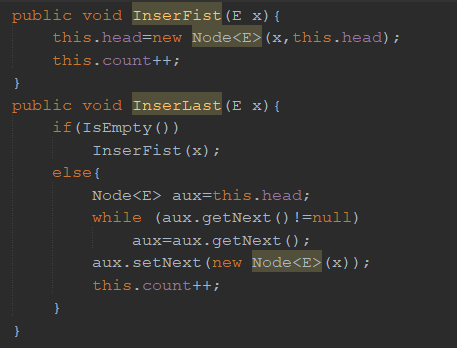
\includegraphics[width=0.6\textwidth,keepaspectratio]{img/insertar.png}\\
			\textbf{Contamos con el m�todo IsEmpty este con la capacidad de mostrar que la lista esta vac�a o por lo menos tiene un elemento, adem�s tenemos el m�todo toString que nos permite mostrar los elementos de nuestra lista enlazada.}\\
			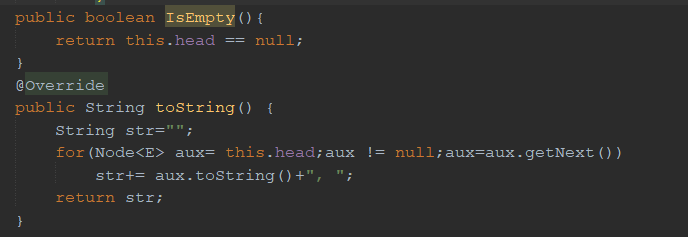
\includegraphics[width=0.6\textwidth,keepaspectratio]{img/verificar.png}\\
			\textbf{Dado que en la informaci�n que se nos muestra en el c�digo que nos da a implementar el ejercicio 1 vemos la capacidad de manipular mediante �ndices.}\\
			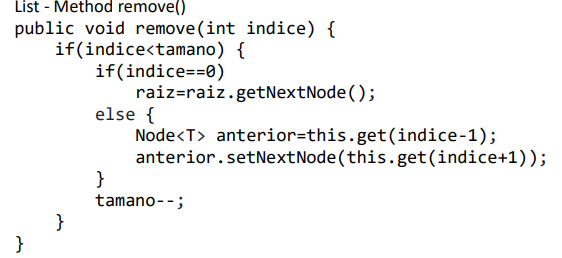
\includegraphics[width=0.9\textwidth,keepaspectratio]{img/remove.png}\\
			\textbf{En nuestra clase main implementamos insertionSort y generarPeorCaso. El m�todo insertionSort solo se ejecutar� siempre y cuando la lista tenga por lo menos un elemento dado a que se habilito la capacidad de usar �ndices modificamos el c�digo dado en la gu�a del laboratorio para que pueda trabajar con una lista enlazada.}\\
			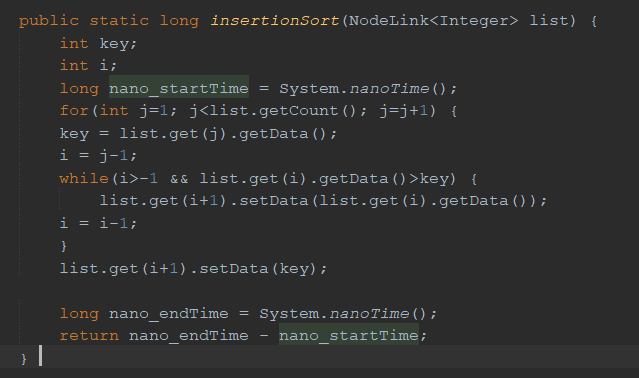
\includegraphics[width=0.9\textwidth,keepaspectratio]{img/insercion.png}\\
			\textbf{Se modifica el m�todo generarPeorCaso para que este retorne una lista enlazada.}\\
			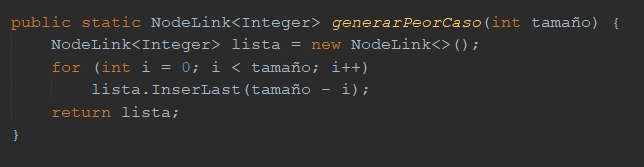
\includegraphics[width=0.6\textwidth,keepaspectratio]{img/peorcaso.png}\\
			\textbf{Se descarg� el proyecto java plot de https://javaplot.yot.is/. Donde se agreg� el ejercicio 1 como eda_lab4_ej1 importando JavaPlot.}\\
			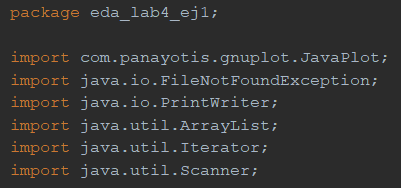
\includegraphics[width=0.6\textwidth,keepaspectratio]{img/importar.png}\\
			\textbf{Al ejecutarlo con 1000 nodos quedo el siguiente gr�fico.}\\
			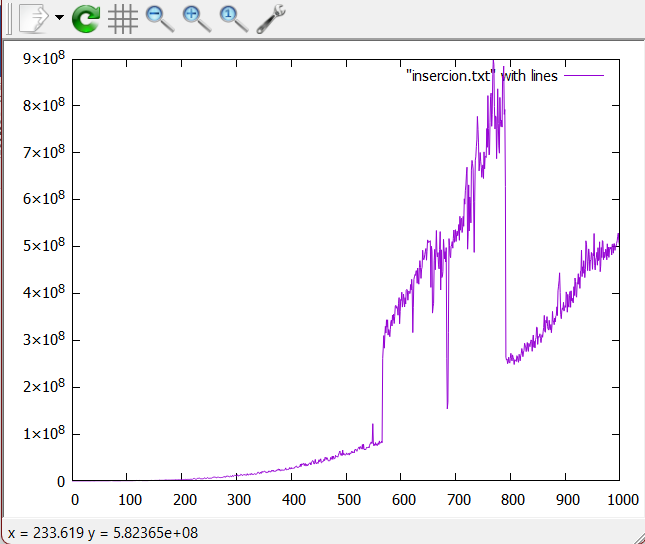
\includegraphics[width=0.8\textwidth,keepaspectratio]{img/grafico.png}\\
			\textbf{Ejercicio 2}  \\
			\textbf{Para lograr ejecutar el algoritmo de ordenamiento por insercion 
			primero fue necesario crear la clase ListaDoble el cual tenia 2 nodos,
			uno inicial y otro final. Con esto se lograba recorrer la lista de el
			fin al inicio y en viceverza.}  \\
			\textbf{El metodo addFinal permitia insertar un nodo al final y el otro
			metodo addInicio, al inicio, dependeiendo si es que estaba vacia o no la lista.}  \\
			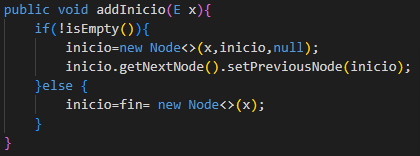
\includegraphics[width=0.6\textwidth,keepaspectratio]{img/addInicio.png}\\
			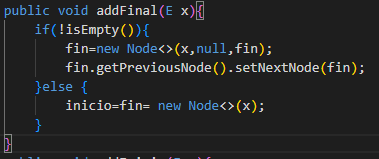
\includegraphics[width=0.6\textwidth,keepaspectratio]{img/addFinal.png}\\
			\textbf{Asismimo se agrego el metodo isEmpty para saber si estaba vacia 
			y se sobreescribio el metodo toString para mostrar retornar la data 
			del 1er al ultimo nodo. Los getters y setters se omitieron en la imagen.}\\
			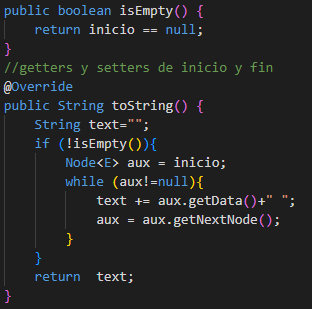
\includegraphics[width=0.6\textwidth,keepaspectratio]{img/otros.png}\\
			\textbf{Se creo la clase Test  para implementar el insertionSort y generarPeorCaso.
			El metodo insertionSort se modifico haciendo que se verificara si es que 
			la lista no estuviera vacia y en caso fuera asi recorria con un 
			for en ves de un while hasta que el nodo siguiente fuera nulo. Dentro de este while
			habia otro que intercambiaba la data, en este caso Integer, de los nodos
			haciendo que los menores quedaran al inicio y los mayores al final. Retornaba
			el tiempo que se demoraba haciendo la operacion.}\\
			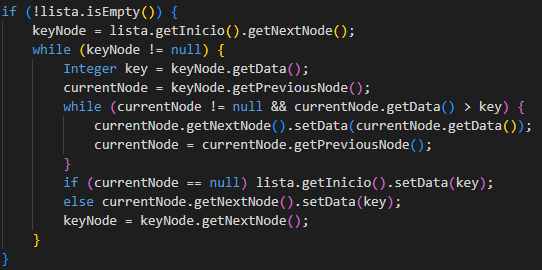
\includegraphics[width=0.9\textwidth,keepaspectratio]{img/insertionSort.png}\\
			\begin{lstlisting}[language=Java,caption={Retorno de insertionSort}][H]
				return nano_endTime - nano_startTime;
			\end{lstlisting}\\
			\textbf{El metodo generarPeorCaso se modifico para que retornara una ListaDoble donde su
			primer elemento fuera el tamanio-1 y el ultimo 1, donde tamanio era el valor que 
			se recibia por argumento, quedando asi el peor caso para hacer insertionSort.}\\
			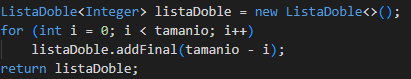
\includegraphics[width=0.6\textwidth,keepaspectratio]{img/generador.png}\\
			\textbf{Por ultimo se descargo el proyecto java plot de \url{https://javaplot.yot.is/}.
			Donde se agrego ejercicio 2 como e2 importando JavaPlot con ayuda de [,] para
			saber coo usarla y agregarlo a mi ide respectivamente.}\\
			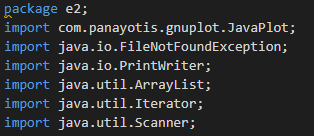
\includegraphics[width=0.6\textwidth,keepaspectratio]{img/importaciones.png}\\
			\textbf{Al ejecutarlo con 1000 nodos quedo el siguiente grafico, donde en el
			eje x es el numero de nodos y en el y el tiempo en nanosegundos que tomo ordenarlo.
			Nanosegundos = 10 elevado a -7 segundos.}\\
			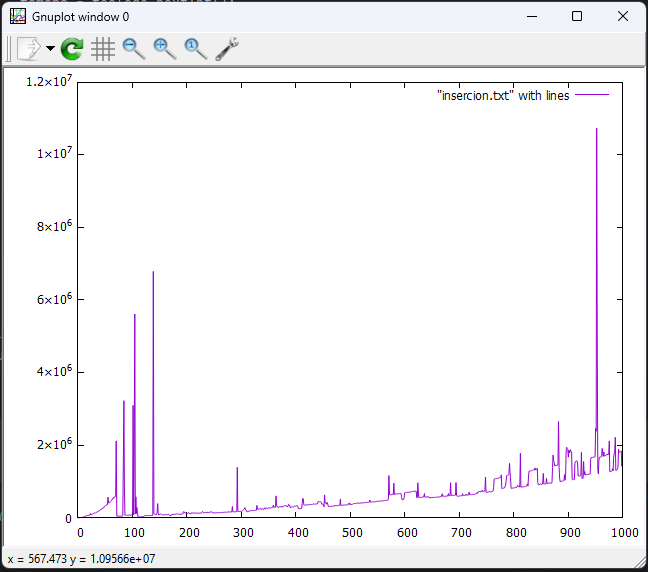
\includegraphics[width=0.8\textwidth,keepaspectratio]{img/plot.png}\\
			\hline
			%%%%%%%%%%%%			
	\end{longtable}
	%%%%%%%%%%%%%%%%%%%%%%%%
	\begin{table}[H]
		\begin{tabular}{|p{15cm}|}
			\hline 
			\rowcolor{tablebackground}
			\color{white}\textbf{LECCIONES APRENDIDAS Y CONCLUSIONES}  \\
			\hline 
			\textbf{Se aprendio que es el metodo de ordenamiento por insercion, 
			al igual que como implementarlo para Listas simples y dobles. Por otro lado se
			a crear los peores casos para este ordenamiento y a como guardar los resultados
			hasta n casos. Con esto se uso JavaPlot para graficar los resultados,
			como se muestran en el ejercicio 1 y 2.}  \\
			\hline 
			%%%%%%%%%%%%
			\rowcolor{tablebackground}
			\color{white}\textbf{REFERENCIAS Y BIBLIOGRAFÍA}  \\
			\hline 
			\textbf{[]\url{https://www.youtube.com/watch?v=35zTmB9HB6g}}\\
			\textbf{[]\url{https://www.youtube.com/watch?v=7wDeHDASoSw}}\\
			\hline 
			%%%%%%%%%%%%			
		\end{tabular}
	\end{table}
	%%%%%%%%%%%%%%%%%%%%%%%%
\end{document}
